\documentclass[a4paper, 11pt]{article}
\usepackage{comment} 
\usepackage{fullpage} 
\usepackage[spanish]{babel} 
\selectlanguage{spanish}
\usepackage[utf8]{inputenc}
\usepackage{float} 
\usepackage{graphicx}
\usepackage{ marvosym }
\usepackage{amsthm}
\usepackage{amsmath}
\usepackage[sort&compress, numbers]{natbib}
\usepackage{amssymb}
\usepackage{hyperref}
%\hypersetup{colorlinks=True, citecolor=blue}
\hypersetup{colorlinks=true, citecolor=green, urlcolor=blue}

\begin{document}
\begin{center}
\LARGE \bf Pr\'actica 11\\ Frentes de Pareto
\end{center}

\vspace{1cm} 
\noindent\textbf {Edson Edgardo Samaniego Pantoja} \hfill \textbf{Materia:} Simulación computacional 
\hfill \\
\textbf{Fecha} \today  
\vspace{1cm} 

\section{Introducción}
En la práctica se trabaja con optimización multicriterio, mejor explicado trata de que a un problema con múltiples objetivos, en donde estos objetivos pueden contraponerse, mientras uno mejora los otros empeoran y viceversa. 

\section{Objetivo}
El objetivo es graficar el porcentaje de soluciones de Pareto como función del número de funciones objetivo para $\texttt{k} \in \left[ 2, 8 \right]$ en pasos de dos y estos datos ser visualizados en diagramas de violín combinado con diagrama caja-bigote.

\section{Simulación}
El código base es dado en el repositorio de Schaeffer \cite{elisa} que de igual manera se puede consultar en la pagina web \cite{dra} donde se explica cada código paso a paso.
Primeramente la modificación realizada en el programa es hacer variante la variable \texttt{k} la cual manda la cantidad de número de funciones objetivo.

\begin{verbatim}
for k in range(2, 9, 2):
    n = 500 # cuantas soluciones aleatorias
    replicas=30
    porcentaje=[]
    for rep in range(0, replicas):
        obj = [poli(md, vc, tc) for i in range(k)]
        minim = np.random.rand(2) > 0.5
        sol = np.random.rand(n, vc)
        val = np.zeros((n, 2))
\end{verbatim}
Como se puede observar se utiliza un ciclo \texttt{for} que toma valores de dos a nueve en saltos de dos y posteriormente entra a otro ciclo \texttt{for} el cual genera réplicas (treinta) del programa que realiza la obtención de los mejores resultados conocidos como frentes de Pareto.

Los mejores resultados de las treinta réplicas son convertidas a un porcentaje respectivo a las soluciones aleatorias dadas en la variable \texttt{n} de valor quinientos para poder almacenarlo en una lista llamada \texttt{porcentaje}.


\begin{verbatim}
        for i in range(n): 
            for j in range(2):
                val[i, j] = evaluate(obj[j], sol[i])
        sign = [1 + -2 * m for m in minim]
        mejor1 = np.argmax(sign[0] * val[:, 0])
        mejor2 = np.argmax(sign[1] * val[:, 1])
        cual = {True: 'min', False: 'max'}

        dom = []
        for i in range(n):
            d = [domin_by(sign * val[i], sign * val[j]) for j in range(n)]  
            dom.append(sum(d))
        frente = val[[d == 0 for d in dom], :]
        porc=(len(frente)*100)/n
        porcentaje.append(porc)
    pc_violin.append(porcentaje)
\end{verbatim}

La lista indexada de treinta porcentajes es acumulada en otra lista \texttt{pcviolin} que acumula por cada función objetivo, de esta manera se tiene una lista de listas de porcentajes por función objetivo. El programa puede ser consultado en github \cite{Edson}.

\section{Resultados}
Los resultados a graficar mostrados en la figura \ref{f1} son tomados de la lista de listas donde se acumuló los porcentajes de cada función objetivo para de esa manera poder generar los diagramas de violín que muestran la diferencia entre cada una de las funciones.


\begin{figure}[H]
  \centering      
  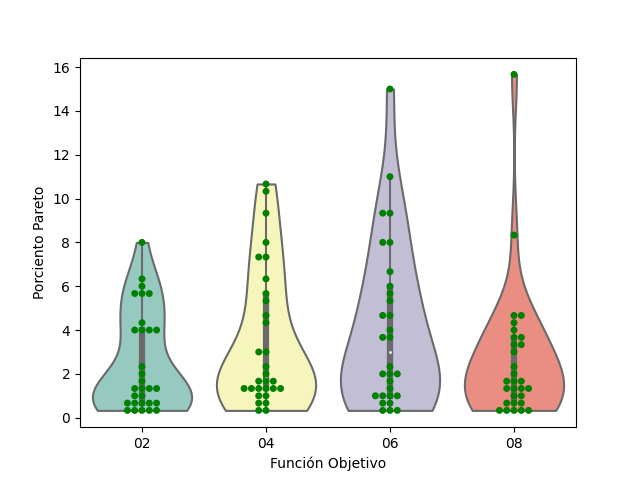
\includegraphics[scale=.8]{diag_violin_300.png}
  \caption{Diagrama violín por función de objetivo contra el porcentaje de resultados de Pareto}
  \label{f1}
\end{figure}
\bigskip

\section{Conclusión}
Como conclusión en base a la figura \ref{f1} se puede ver que los puntos comienzan distribuidos a lo largo del violín pero no llegan a más de ocho porciento y conforme aumenta la función objetivo la cantidad de porcentajes comienza a bajar para asentarse en la parte inferior pero llega a haber porcentajes que llegan más lejos (dieciséis porciento) aunque no sean muchos. 

\bibliography{refe}
\bibliographystyle{plainnat}

\end{document}
